
%{
%\setbeamertemplate{headline}{}
%\setbeamertemplate{footline}{}
%\usebackgroundtemplate{
%  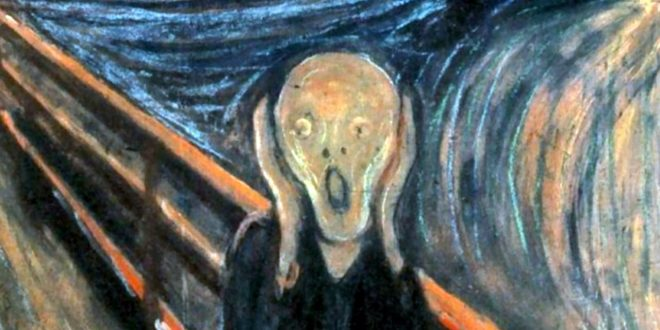
\includegraphics[width=\paperwidth]{munch2.jpg}
%}
%\begin{frame}
%\end{frame}
%}

%\section{Введение в Haskell}


%\defverbatim[colored]{\imageA}{
%\begin{tikzpicture}
%    [%%%%%%%%%%%%%%%%%%%%%%%%%%%%%%
%        box/.style={rectangle,draw=black, ultra thick, minimum size=1cm},
%    ]%%%%%%%%%%%%%%%%%%%%%%%%%%%%%%
%
%\foreach \x/\y in {0/9, 1/\faAmazon,2/13,3/19,4/12,5/8,6/7,7/4,8/21,9/2,10/6,11/11}
%        \node[box] at (\x,0){\y};
%
%\end{tikzpicture}
%}


\begin{frame}{Введение}
\begin{center}
\only<1>{
\includegraphics{tikzpics/array1.pdf}
}
\only<2>{
\includegraphics{tikzpics/array2.pdf}
}
\only<3>{
\includegraphics{tikzpics/array1.pdf}
}
\only<4>{
\includegraphics{tikzpics/array1.pdf}
\vspace{2em}

\includegraphics{tikzpics/array2.pdf}
}
\end{center}
\end{frame}

\begin{frame}{Чистые функции}
\begin{definition}{Чистая функция -- это}
  \begin{itemize}
    \item Детерминированная
    \item В процессе работы не совершающая ``побочных эффектов''
  \end{itemize}
\end{definition}
Т.е. запрещены: ввод-вывод, случайные значения, присваивания\\

N.B. Это свойство \emph{функции}, а не языка программирования
\end{frame}

\begin{frame}%{Чистые функции}
\begin{definition}[Неизменяемые структуры данных (immutable data structures)]
  Которые с течением времени не изменяются \faSmileO
\end{definition}

\vspace{1em}

\begin{definition}[Устойчивые структуры данных (persistent data structures)]
Имеют доступ (не уничтожают) предыдущее своё состояние
\end{definition}
Почти то же самое, только акцент смещён\vspace{1em}

\begin{remark}
Так как старые узлы есть, то можно их использовать (share) в новой версии структуры данных
\end{remark}
\begin{definition}[Неустойчивые структуры данных называются \textit{эфемерными (ephemeral)}]
\end{definition}
\end{frame}

